\documentclass[chaptersright]{informeutn}
\usepackage{tikz}
\usetikzlibrary{plotmarks}
\usepackage{pgfplots}
\pgfplotsset{compat=1.18}
\usepackage{caption}
\captionsetup{justification=centering}
\usepackage{graphicx}
\usepackage{circuitikz}

% Datos del informe
\materia{Electronica Aplicada}
\titulo{Trabajo Práctico 1}
\comision{3R2}
\autores{
          Gaston Grasso - 401892\\
          Franco Palombo - 401910\\
          Angelo Prieto - 401012}
\fecha{1-1-1}

\begin{document}
  \maketitle

  \tableofcontents
  \setcounter{page}{1}
  \thispagestyle{plain}git@github.com:fpp3/ElectronicaAplicada1.git

  \chapter{Introducción} 

    En el marco de la asignatura \textit{Electrónica Aplicada I}, se llevó a cabo un trabajo práctico centrado en la
    construcción y análisis de una fuente de alimentación de tensión variable. Este tipo de fuente resulta fundamental
    en entornos de laboratorio y desarrollo electrónico, ya que permite alimentar circuitos con distintos
    requerimientos de tensión de forma estable y segura.

    El diseño de la fuente fue provisto por el docente a cargo, por lo que el enfoque del trabajo no estuvo en la etapa
    de diseño conceptual, sino en la interpretación, armado y validación funcional del circuito. La actividad comenzó
    con una clase teórica introductoria, donde se abordaron los fundamentos técnicos del proyecto y se detallaron los
    criterios de análisis a aplicar en laboratorio. Al finalizar la clase, el docente realizó la entraga de los 
    materiales necesarios para avanzar con la construcción.

    La realización del proyecto se desarrolló de manera progresiva, abordando dos etapas principales de la
    fuente, primero: transformación, rectificación y filtrado; luego regulación. Esta metodología permitió realizar 
    ensayos parciales, facilitando la comprensión del comportamiento eléctrico en cada etapa.

    El circuito final tiene la capacidad de entregar una tensión de salida variable entre 0 y 30\,V con una corriente
    máxima de 1.5\,A. Se efectuaron ensayos destinados a verificar su desempeño, incluyendo mediciones de
    \textit{ripple}, control de regulación de voltaje, y análisis de temperatura en el regulador LM317. Más allá de su
    valor académico, la fuente construida será utilizada como herramienta de alimentación en futuros trabajos
    prácticos, reafirmando así su utilidad práctica y formativa.

  \chapter{Planeamiento e introduccion teorica}
    A continuación se va a explicar el funcionamiento de cada uno de los siguientes bloques de la fuente:
    \begin{itemize}
      \item Transformador.
      \item Rectificacion.
      \item Filtrado.
      \item Regulacion.
      \item Otros.
    \end{itemize}
        
      \section{Transformador}
        El transformador cumple dos funciones principales:
        \begin{itemize}
          \item Proporciona aislamiento galvanico entre la red de 220 V y la fuente mediante acoplamiento magnetico.
          \item Reduce la tension de 220 V a un valor adecuado (como 12 V o 24 V) segun las necesidades de la fuente.
        \end{itemize}
        A continuacion, un esquematico del transformador:
        

        \begin{figure}[h]
          \centering
          \includegraphics[width=0.5\textwidth]{imagenes/Sch_Trafo.png}
          \caption{Texto de la leyenda (caption)}
          \label{fig:etiqueta}
        \end{figure}

      \section{Rectificacion}
        La función del rectificador es convertir la tensión alterna en una continua pulsante, el circuito siguiente 
        realiza esa función y se lo conoce como puente de diodos, previamente vemos el comportamiento de un diodo 
        individual.
        El rectificador se encarga de convertir la onda senoidal alterna en una continua pulsante. El protagonista
        principal es el puente de diodos.

              \section{filtrado}

  \chapter{Ensayos y mediciones}
  
    Posterior al armado de la placa hasta la etapa de filtrado (sin regulación), es decir, hasta el montaje del
    puente de diodos y los correspondientes componentes de filtrado, se procedió al ensayo de la misma. Con esto,
    podríamos determinar los parámetros de operación que permitirán al regulador integrado trabajar con seguridad,
    el cual forma parte de la siguiente etapa.

    \section{Fuente no regulada}
    
     \subsection{Medición de ripple} 
        
        El transformador que se utiliza para bajar la tensión alterna de 220V a 12+12v, consta de dos bobinados que 
        proporcionan 12v cada uno. Por lo
        tanto el ensayo de la placa se realizó en dos apartados; una en el punto bajo de la fuente utilizando un solo
        bobinado del transformador (12v) y, otro en el punto alto de la fuente utilizando los dos bobinados (24v). En
        ambos casos se ha medido la tensión de salida de la fuente no regulada en vacío, y luego se ha conectado a la
        misma una carga variable (reostato) para analizar qué tensión otorga la fuente según la corriente que pasa por
        la carga, hasta un máximo de 1.5A. Con estos datos podríamos calcular la resistencia interna del transformador
        más la de los diodos, el factor de ripple, etc.
        
        Las mediciones tomadas y los cálculos correspondientes se muestran a continuación:

        \subsubsection{Punto bajo}
        
        \begin{figure}[H]
        % Minipage para la tabla
        \begin{minipage}{0.35\textwidth}
        \centering
        \begin{tabular}{|c|c|}
        \hline
        $I_{out}$ [A] & $V_{out}$ [V] \\
        \hline
        0.00 & 17.65 \\
        0.50 & 15.45 \\
        0.75 & 14.82 \\
        1.00 & 14.24 \\
        1.25 & 13.64 \\
        1.50 & 13.16 \\
        \hline
        \end{tabular}
        \end{minipage}
        \begin{minipage}{0.35\textwidth}
        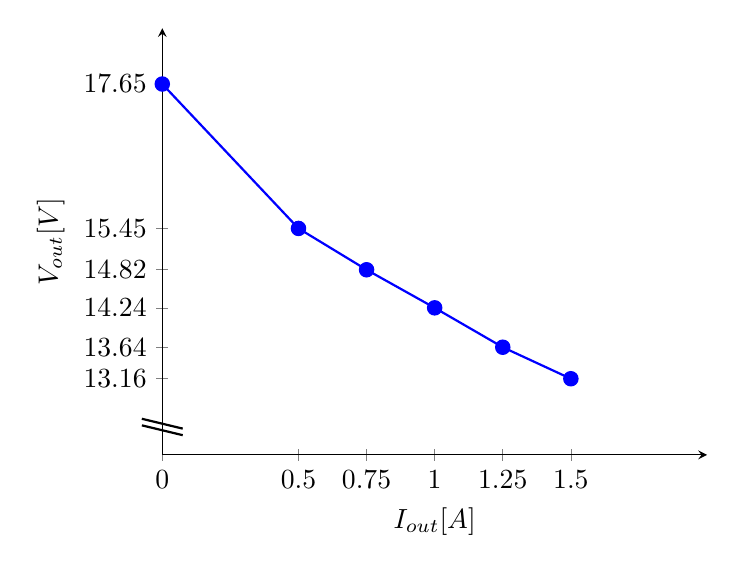
\begin{tikzpicture}
          \begin{axis}[
            axis lines = left,
            xlabel = {$I_{out}[A]$},
            ylabel = {$V_{out}[V]$},
            width=8.5cm,
            height=7cm,
            ymin=12, ymax=18.5,
            xmin=0, xmax=2,
            ytick={13.16,13.64,14.24,14.82,15.45,17.65},
            xtick={0,0.5,0.75,1,1.25,1.5},
            clip=false, % necesario para dibujar fuera del área del gráfico
          ]
            % Puntos conectados por líneas
            \addplot[
              color=blue,
              mark=*,
              only marks,
              mark options={scale=1.3}
            ]
            coordinates {
              (0,17.65)(0.5,15.45) (0.75,14.82) (1.00,14.24) (1.25,13.64) (1.5,13.16)
            };
            
            \addplot[
              color=blue,
              thick
            ]
            coordinates {
              (0,17.65)(0.5,15.45) (0.75,14.82) (1.00,14.24) (1.25,13.64) (1.5,13.16)
            };
            \draw[thick]
              (axis cs:0.075,12.3) -- ++(-0.15,12.15);
            \draw[thick]
              (axis cs:0.075,12.4) -- ++(-0.15,12.15);
          \end{axis}
        \end{tikzpicture}
        \end{minipage}%
        \caption{\footnotesize
        Tensión de salida de la fuente $V_{out}$ (punto bajo) en función \\
        de la corriente $I_{out}$ sobre una carga variable}
        \label{fig:curva_salida_bajo}
        \end{figure}
        
        Para calcular la resistencia interna se considera:

        \begin{equation}
            R_{int} = \frac{V_{vacio} - V_{carga}}{I_{max}}= \frac{17.65V - 13.16V}{1.5A} = 2.99\Omega
        \end{equation}

        Por otro lado, se puede determinar el desempeño de la fuente para mantener la tensión constante frente a
        condiciones sin carga y con carga máxima mediante el siguiente cálculo:

        \begin{equation}
            RV = \frac{V_{vacio} -V_{carga}}{V_{carga}} \times 100\% = \frac{17.65V-13.16V}{13.16V} \times 100\% = 34.1185\%
        \end{equation}
        
        Finalmente, el factor de ripple, que es un indicador de la efectividad del filtro se define como:

        \begin{equation}
            FR = \frac{V_{eficaz-ripple}}{V_{carga}} \times 100\%
        \end{equation}

        El $V_{eficaz-ripple}$ es la tensión medida con el multimétro establecido en escala de tensión alterna.
        Para ello, nos aseguramos de que el multimétro mida valor verdadero eficaz (true RMS) para realizar una
        medición más acertada. Considerando entonces el valor de $V_{eficaz-ripple}$ medido:

        \begin{equation}
            FR = \frac{0.873V}{13.16V} \times 100\% = 6.6337\%
        \end{equation}

        \subsubsection{Punto alto}
        \begin{figure}[H]

        % Minipage para la tabla
        \begin{minipage}{0.35\textwidth}
        \centering
        \begin{tabular}{|c|c|}
        \hline
        $I_{out}$ [A] & $V_{out}$ [V] \\
        \hline
        0.00 & 36.75 \\
        0.50 & 31.51 \\
        0.75 & 30.37\\
        1.00 & 28.92 \\
        1.25 & 27.76 \\
        1.50 & 26.62 \\
        \hline
        \end{tabular}
        \end{minipage}
        \begin{minipage}{0.35\textwidth}
        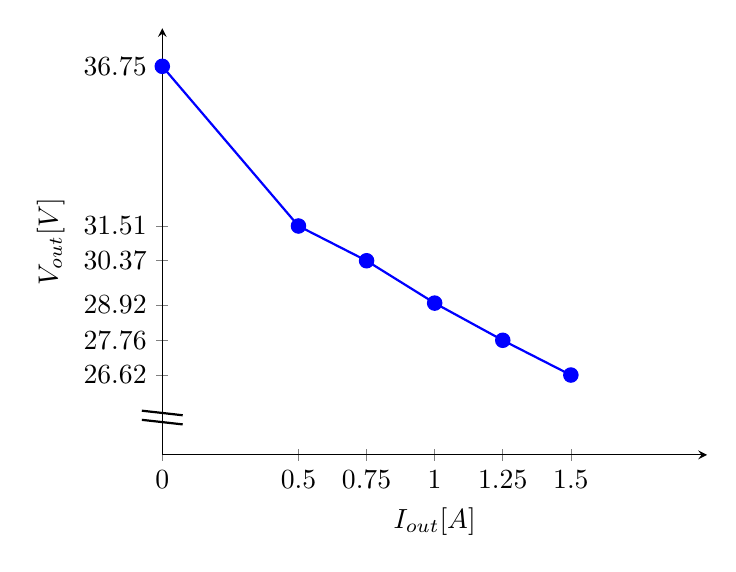
\begin{tikzpicture}
          \begin{axis}[
            axis lines = left,
            xlabel = {$I_{out}[A]$},
            ylabel = {$V_{out}[V]$},
            width=8.5cm,
            height=7cm,
            ymin=24, ymax=38,
            xmin=0, xmax=2,
            ytick={26.62,27.76,28.92,30.37,31.51,36.75},
            xtick={0,0.5,0.75,1,1.25,1.5},
            clip=false, % necesario para dibujar fuera del área del gráfico
          ]
            % Puntos conectados por líneas
            \addplot[
              color=blue,
              mark=*,
              only marks,
              mark options={scale=1.3}
            ]
            coordinates {
              (0,36.75)(0.5,31.51) (0.75,30.37) (1.00,28.98) (1.25,27.76) (1.5,26.62)
            };
            
            \addplot[
              color=blue,
              thick
            ]
            coordinates {
              (0,36.75)(0.5,31.51) (0.75,30.37) (1.00,28.98) (1.25,27.76) (1.5,26.62)
            };
            \draw[thick]
              (axis cs:0.075,25) -- ++(-0.15,24.15);
            \draw[thick]
              (axis cs:0.075,25.3) -- ++(-0.15,24.15);
          \end{axis}
        \end{tikzpicture}
        \end{minipage}%
        \caption{\footnotesize
        Tensión de salida de la fuente $V_{out}$ (punto alto) en función \\
        de la corriente $I_{out}$ sobre una carga variable}
        \label{fig:curva_salida_alto}
        \end{figure}

        Se calcula nuevamente la resistencia interna, ya que al utilizar los dos bobinados del transformador, ésta
        debe ser algo mayor:

        \begin{equation}
            R_{int} = \frac{V_{vacio} - V_{carga}}{I_{max}}= \frac{36.75V - 26.62V}{1.5A} = 6.7533\Omega
        \end{equation}

        El desempeño de la fuente en el punto alto para mantener la tensión constante en distintas condiciones (sin carga
        y con carga máxima) es:

        \begin{equation}
            RV = \frac{V_{vacio} -V_{carga}}{V_{carga}} \times 100\% = \frac{36.75V-26.62V}{26.62V} \times 100\% = 38.0541\%
        \end{equation}

        El factor de ripple en este caso, con un $V_{eficaz-ripple}=0.812V$ medido es:

        \begin{equation}
            FR = \frac{V_{eficaz-ripple}}{V_{carga}} \times 100\% = \frac{0.812V}{26.62V} \times 100\% = 3.0503\%
        \end{equation}

        \section{Fuente regulada} 

  \chapter{Conclusiones}

\end{document}
